\documentclass[12pt,border=0pt]{standalone}

\usepackage[utf8]{inputenc} 
\usepackage{amssymb,amsmath}
\usepackage{tikz}
\usetikzlibrary{shapes}
\usetikzlibrary{positioning}

\definecolor{aliceblue}{rgb}{0.94, 0.97, 1.0}
\definecolor{aquamarine}{rgb}{0.5, 1.0, 0.83}


\thispagestyle{empty}

\begin{document}

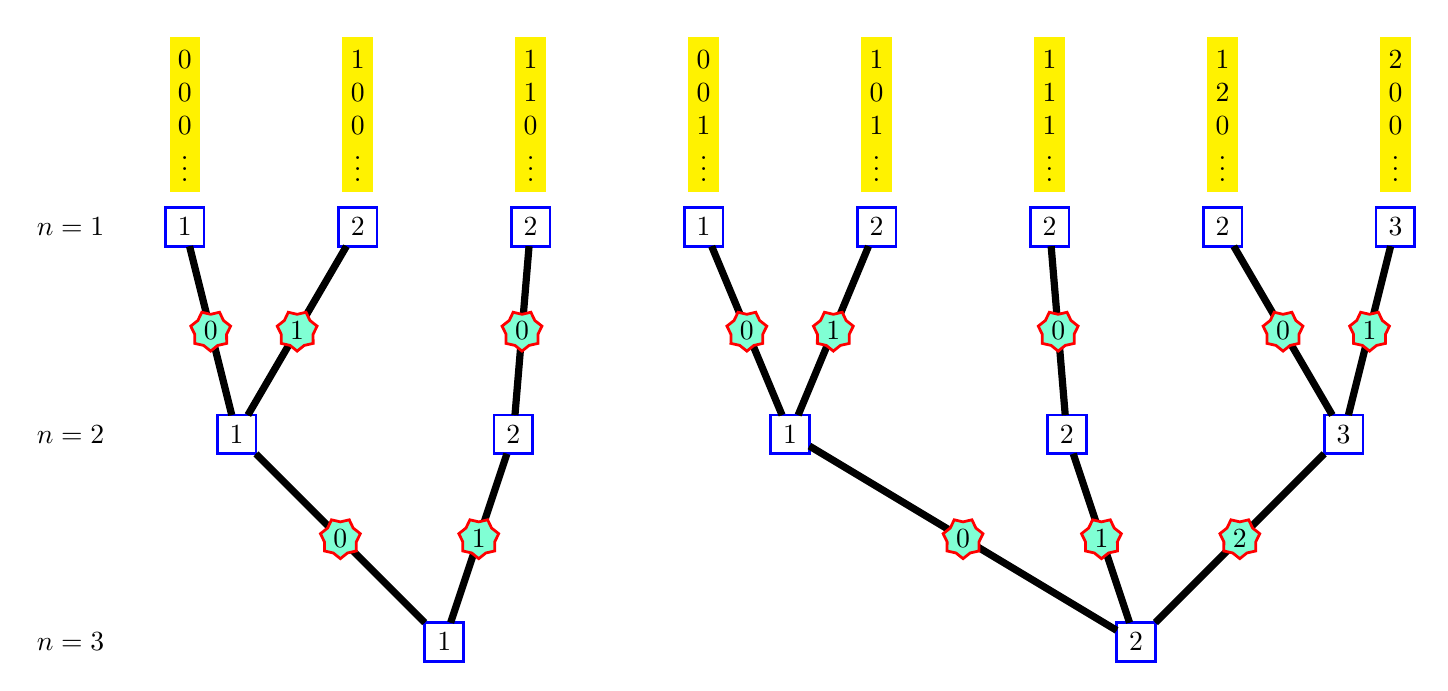
\begin{tikzpicture}[x=10pt,y=6pt]
  \centering
  \tikzset{VertexStyle/.style = {
    shape         = rectangle,
    draw          = blue, 
    fill          = white, 
  	line width    = 1pt, 
    text          = black,
    inner sep     = 1pt,
    outer sep     = 0pt,
    minimum size  = 14 pt,
    scale         = 1
    }
  }
  \tikzset{EdgeStyle/.style = {
    draw            = black, 
    thick,
    double          = black,
    double distance = 1pt
    }
  }
  \tikzset{EdgeLabelStyle/.style = {
    draw          = red,
  	shape         = star,star points=7,star point ratio=0.8, 
  	line width    = 1pt, 
  	minimum size  = 10pt, 
    inner sep     = 2pt,
    outer sep     = 0pt,
    fill          = aquamarine,
    text          = black,
    scale         = 1
    }
  }

	%\node[VertexStyle](A1) at (25, 0) {$\varnothing$};
	\node[VertexStyle](B1) at (12.5, 12.5) {$1$};
	\node[VertexStyle](B2) at (37.5, 12.5) {$2$};
	\node[VertexStyle](C1) at (5, 25) {$1$};
	\node[VertexStyle](C2) at (15, 25) {$2$};
	\node[VertexStyle](C3) at (25, 25) {$1$};
	\node[VertexStyle](C4) at (35, 25) {$2$};
	\node[VertexStyle](C5) at (45, 25) {$3$};
	\node[VertexStyle](D1) at (3.125, 37.5) {$1$};
	\node[VertexStyle](D2) at (9.375, 37.5) {$2$};
	\node[VertexStyle](D3) at (15.625, 37.5) {$2$};
	\node[VertexStyle](D4) at (21.875, 37.5) {$1$};
	\node[VertexStyle](D5) at (28.125, 37.5) {$2$};
	\node[VertexStyle](D6) at (34.375, 37.5) {$2$};
	\node[VertexStyle](D7) at (40.625, 37.5) {$2$};
	\node[VertexStyle](D8) at (46.875, 37.5) {$3$};
	%\draw[EdgeStyle](A1) to node[EdgeLabelStyle]{$0$} (B1);
	%\draw[EdgeStyle](A1) to node[EdgeLabelStyle]{$1$} (B2);
	\draw[EdgeStyle](B1) to node[EdgeLabelStyle]{$0$} (C1);
	\draw[EdgeStyle](B1) to node[EdgeLabelStyle]{$1$} (C2);
	\draw[EdgeStyle](B2) to node[EdgeLabelStyle]{$0$} (C3);
	\draw[EdgeStyle](B2) to node[EdgeLabelStyle]{$1$} (C4);
	\draw[EdgeStyle](B2) to node[EdgeLabelStyle]{$2$} (C5);
	\draw[EdgeStyle](C1) to node[EdgeLabelStyle]{$0$} (D1);
	\draw[EdgeStyle](C1) to node[EdgeLabelStyle]{$1$} (D2);
	\draw[EdgeStyle](C2) to node[EdgeLabelStyle]{$0$} (D3);
	\draw[EdgeStyle](C3) to node[EdgeLabelStyle]{$0$} (D4);
	\draw[EdgeStyle](C3) to node[EdgeLabelStyle]{$1$} (D5);
	\draw[EdgeStyle](C4) to node[EdgeLabelStyle]{$0$} (D6);
	\draw[EdgeStyle](C5) to node[EdgeLabelStyle]{$0$} (D7);
	\draw[EdgeStyle](C5) to node[EdgeLabelStyle]{$1$} (D8);
	
	\node(n3) at (-1, 12.5) {$n=3$};
	\node(n2) at (-1, 25) {$n=2$};
	\node(n1) at (-1, 37.5) {$n=1$};
	
	\node[above=2pt of D1](E1) {\colorbox{yellow}{$\begin{matrix} 0 \\ 0 \\ \underset{\vdots}{0}  \end{matrix}$}} ;
	\node[above=2pt of D2](E2) {\colorbox{yellow}{$\begin{matrix} 1 \\ 0 \\ \underset{\vdots}{0}  \end{matrix}$}} ;
	\node[above=2pt of D3](E3) {\colorbox{yellow}{$\begin{matrix} 1 \\ 1 \\ \underset{\vdots}{0}  \end{matrix}$}} ;
	\node[above=2pt of D4](E4) {\colorbox{yellow}{$\begin{matrix} 0 \\ 0 \\ \underset{\vdots}{1}  \end{matrix}$}} ;
	\node[above=2pt of D5](E5) {\colorbox{yellow}{$\begin{matrix} 1 \\ 0 \\ \underset{\vdots}{1}  \end{matrix}$}} ;
	\node[above=2pt of D6](E6) {\colorbox{yellow}{$\begin{matrix} 1 \\ 1 \\ \underset{\vdots}{1}  \end{matrix}$}} ;
	\node[above=2pt of D7](E7) {\colorbox{yellow}{$\begin{matrix} 1 \\ 2 \\ \underset{\vdots}{0}  \end{matrix}$}} ;
	\node[above=2pt of D8](E8) {\colorbox{yellow}{$\begin{matrix} 2 \\ 0 \\ \underset{\vdots}{0}  \end{matrix}$}} ;	
	\end{tikzpicture}

\end{document}
